\documentclass[a4paper, titlepage, final, 12pt]{article}
\usepackage{graphicx}
\usepackage[czech]{babel}
\usepackage[utf8x]{inputenc}
\usepackage[T1]{fontenc}
\usepackage[a4paper, top=3cm, bottom=2cm, left=3cm, right=3cm, marginparwidth=1.75cm]{geometry}
\usepackage{booktabs}
\usepackage[colorlinks=true, allcolors=blue]{hyperref}

\begin{document}

\def\school{Vysoké učení technické v Brně}
\def\facult{Fakulta informačních techologií}
\def\titleA{Úvod do softwarového inženýrství 2017/2018}
\def\authorA{Jakub Čábera <xcaber00@stud.fit.vutbr.cz>}
\def\project{Projekt IUS --- Model informačního systému}
\def\assignment{Zadání č. 49 --- Bug Tracker}
\def\dateA{\today}

\title{\titleA}
\author{\authorA}
\date{\dateA}

\begin{titlepage}
	\centering{
		
\includegraphics{Logo.png} \\
		\scshape\LARGE \school{} \\
		\scshape\large \facult{} \\
		\vspace{2cm}
		\huge\bfseries \titleA{} \\
		\vspace{4cm}

		\Large \project{} \\
		\vspace{3cm}

		\Large \assignment{} \\

		\vfill
		\large \authorA{} \\
		\dateA{}
	}

\end{titlepage}

\section{Zadání}
	Vytvořte informační systém pro hlášení a správů chyb a zranitelností systému.
	Systém umožňuje uživatelům hlásit bugy, jejich závažnosti a moduly, ve kterých se vyskytly, ve formě tiketů.
	Tikety mohou obsahovat hlášení o více než jednom bugu a stejný bug může být zahlášen více uživateli.
	Bug může (ale nemusí) být zranitelností a v tomto případě zaevidujeme i potenciální míru nebezpečí zneužití této zranitelnosti.
	V případě zahlášení bugů, odešle systém upozornění programátorovi, který zodpovídá za daný modul, přičemž může odpovídat za více modulů. Programátor pak daný tiket zabere, přepne jeho stav na \"V řešení\" a začne pracovat na opravě ve formě Patche.
	Patch je charakterizován datem vydání a musí být schválen programátorem zodpovědným za modul, které mohou být v různých programovacích jazycích. Jeden Patch může řešit více bugů a současně řešit více tiketů a vztahuje se na několik modulů.
	Samotní uživatelé mohou rovněž tvořit patche. Takové patche však musí projít silnější kontrolou než jsou zavedeny do systému. Kromě data vytvoření patche rovněž evidujte datum zavedení patche do ostrého provozu.
	Každý uživatel a programátor je charakterizován základními informacemi (jméno, věk, apod.), ale současně i jazyky, kterými disponuje, apod.
	V případě opravení bugů, mohou být uživatele upozorněni na danou opravu a případně být odměněni peněžní hodnotou (podle závažnosti bugu či zranitelnosti).

\section{Model případů užití}
	\includegraphics[width=\textwidth,height=\textheight,keepaspectratio]{Use-Case.png}

\section{ER diagram}
	\hspace{-1.5cm}
	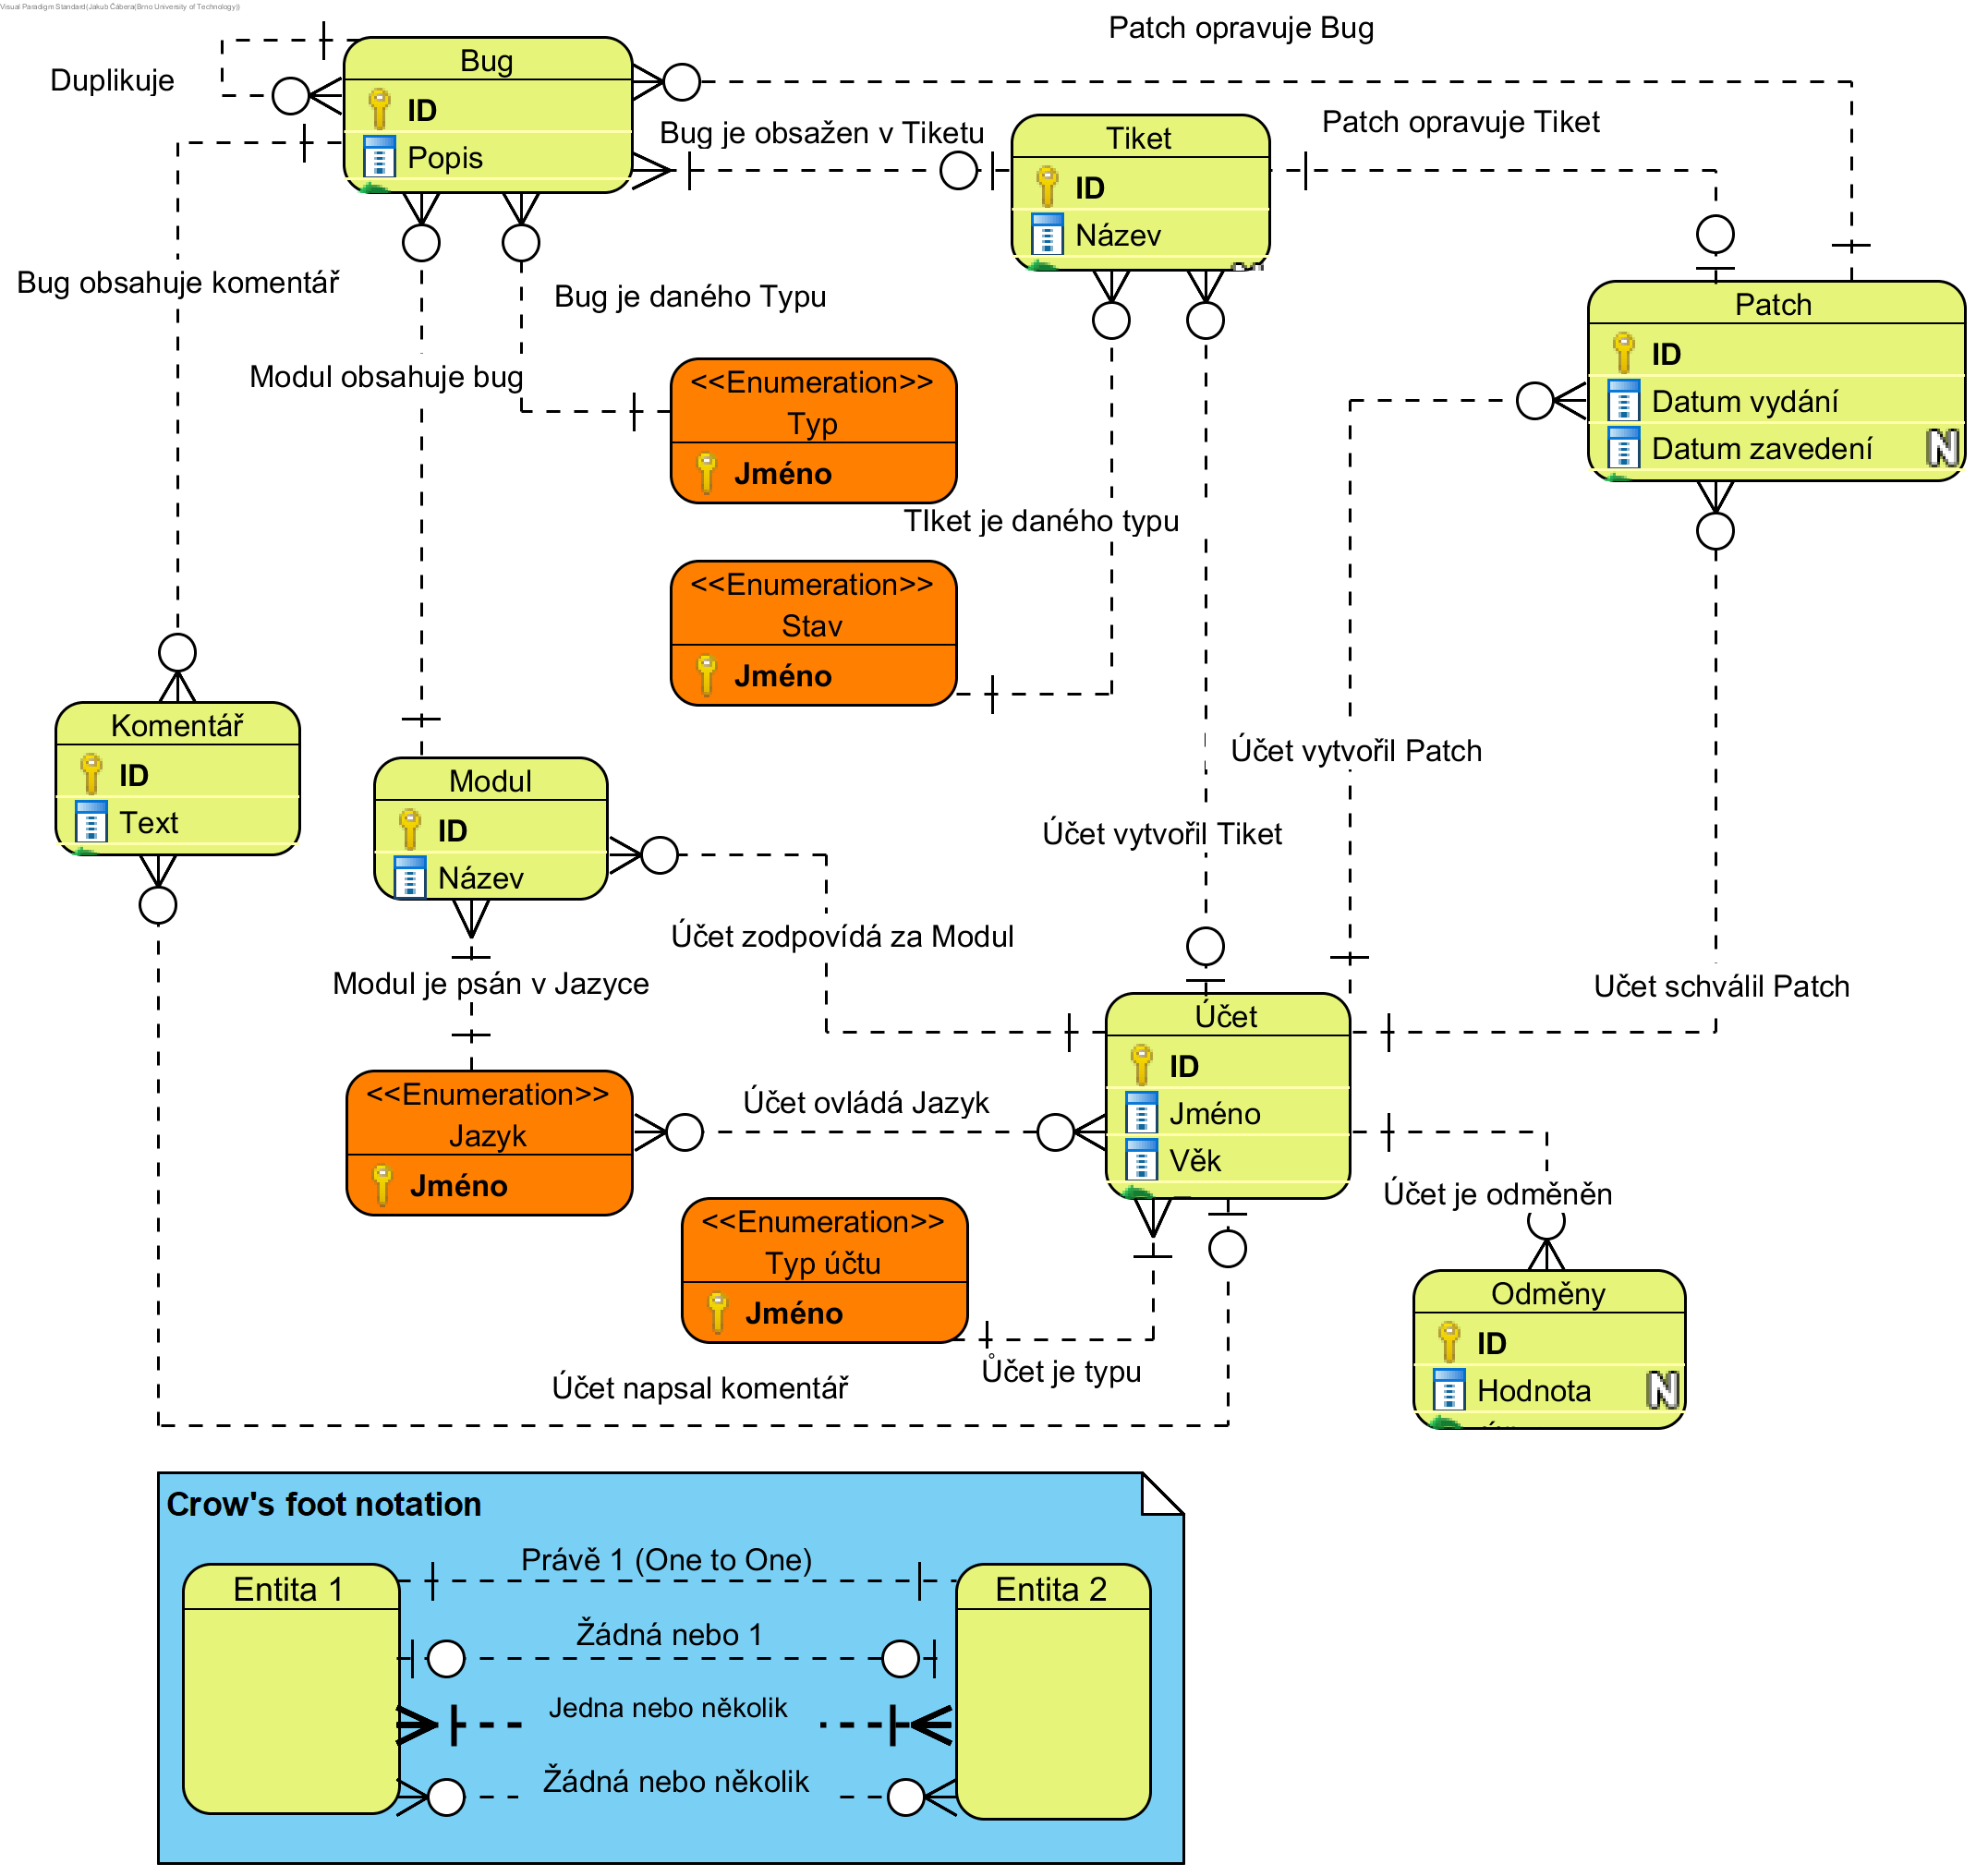
\includegraphics[keepaspectratio]{ER2.png}

\section{ER diagram s cizími klíči}
	\hspace{-1.5cm}
	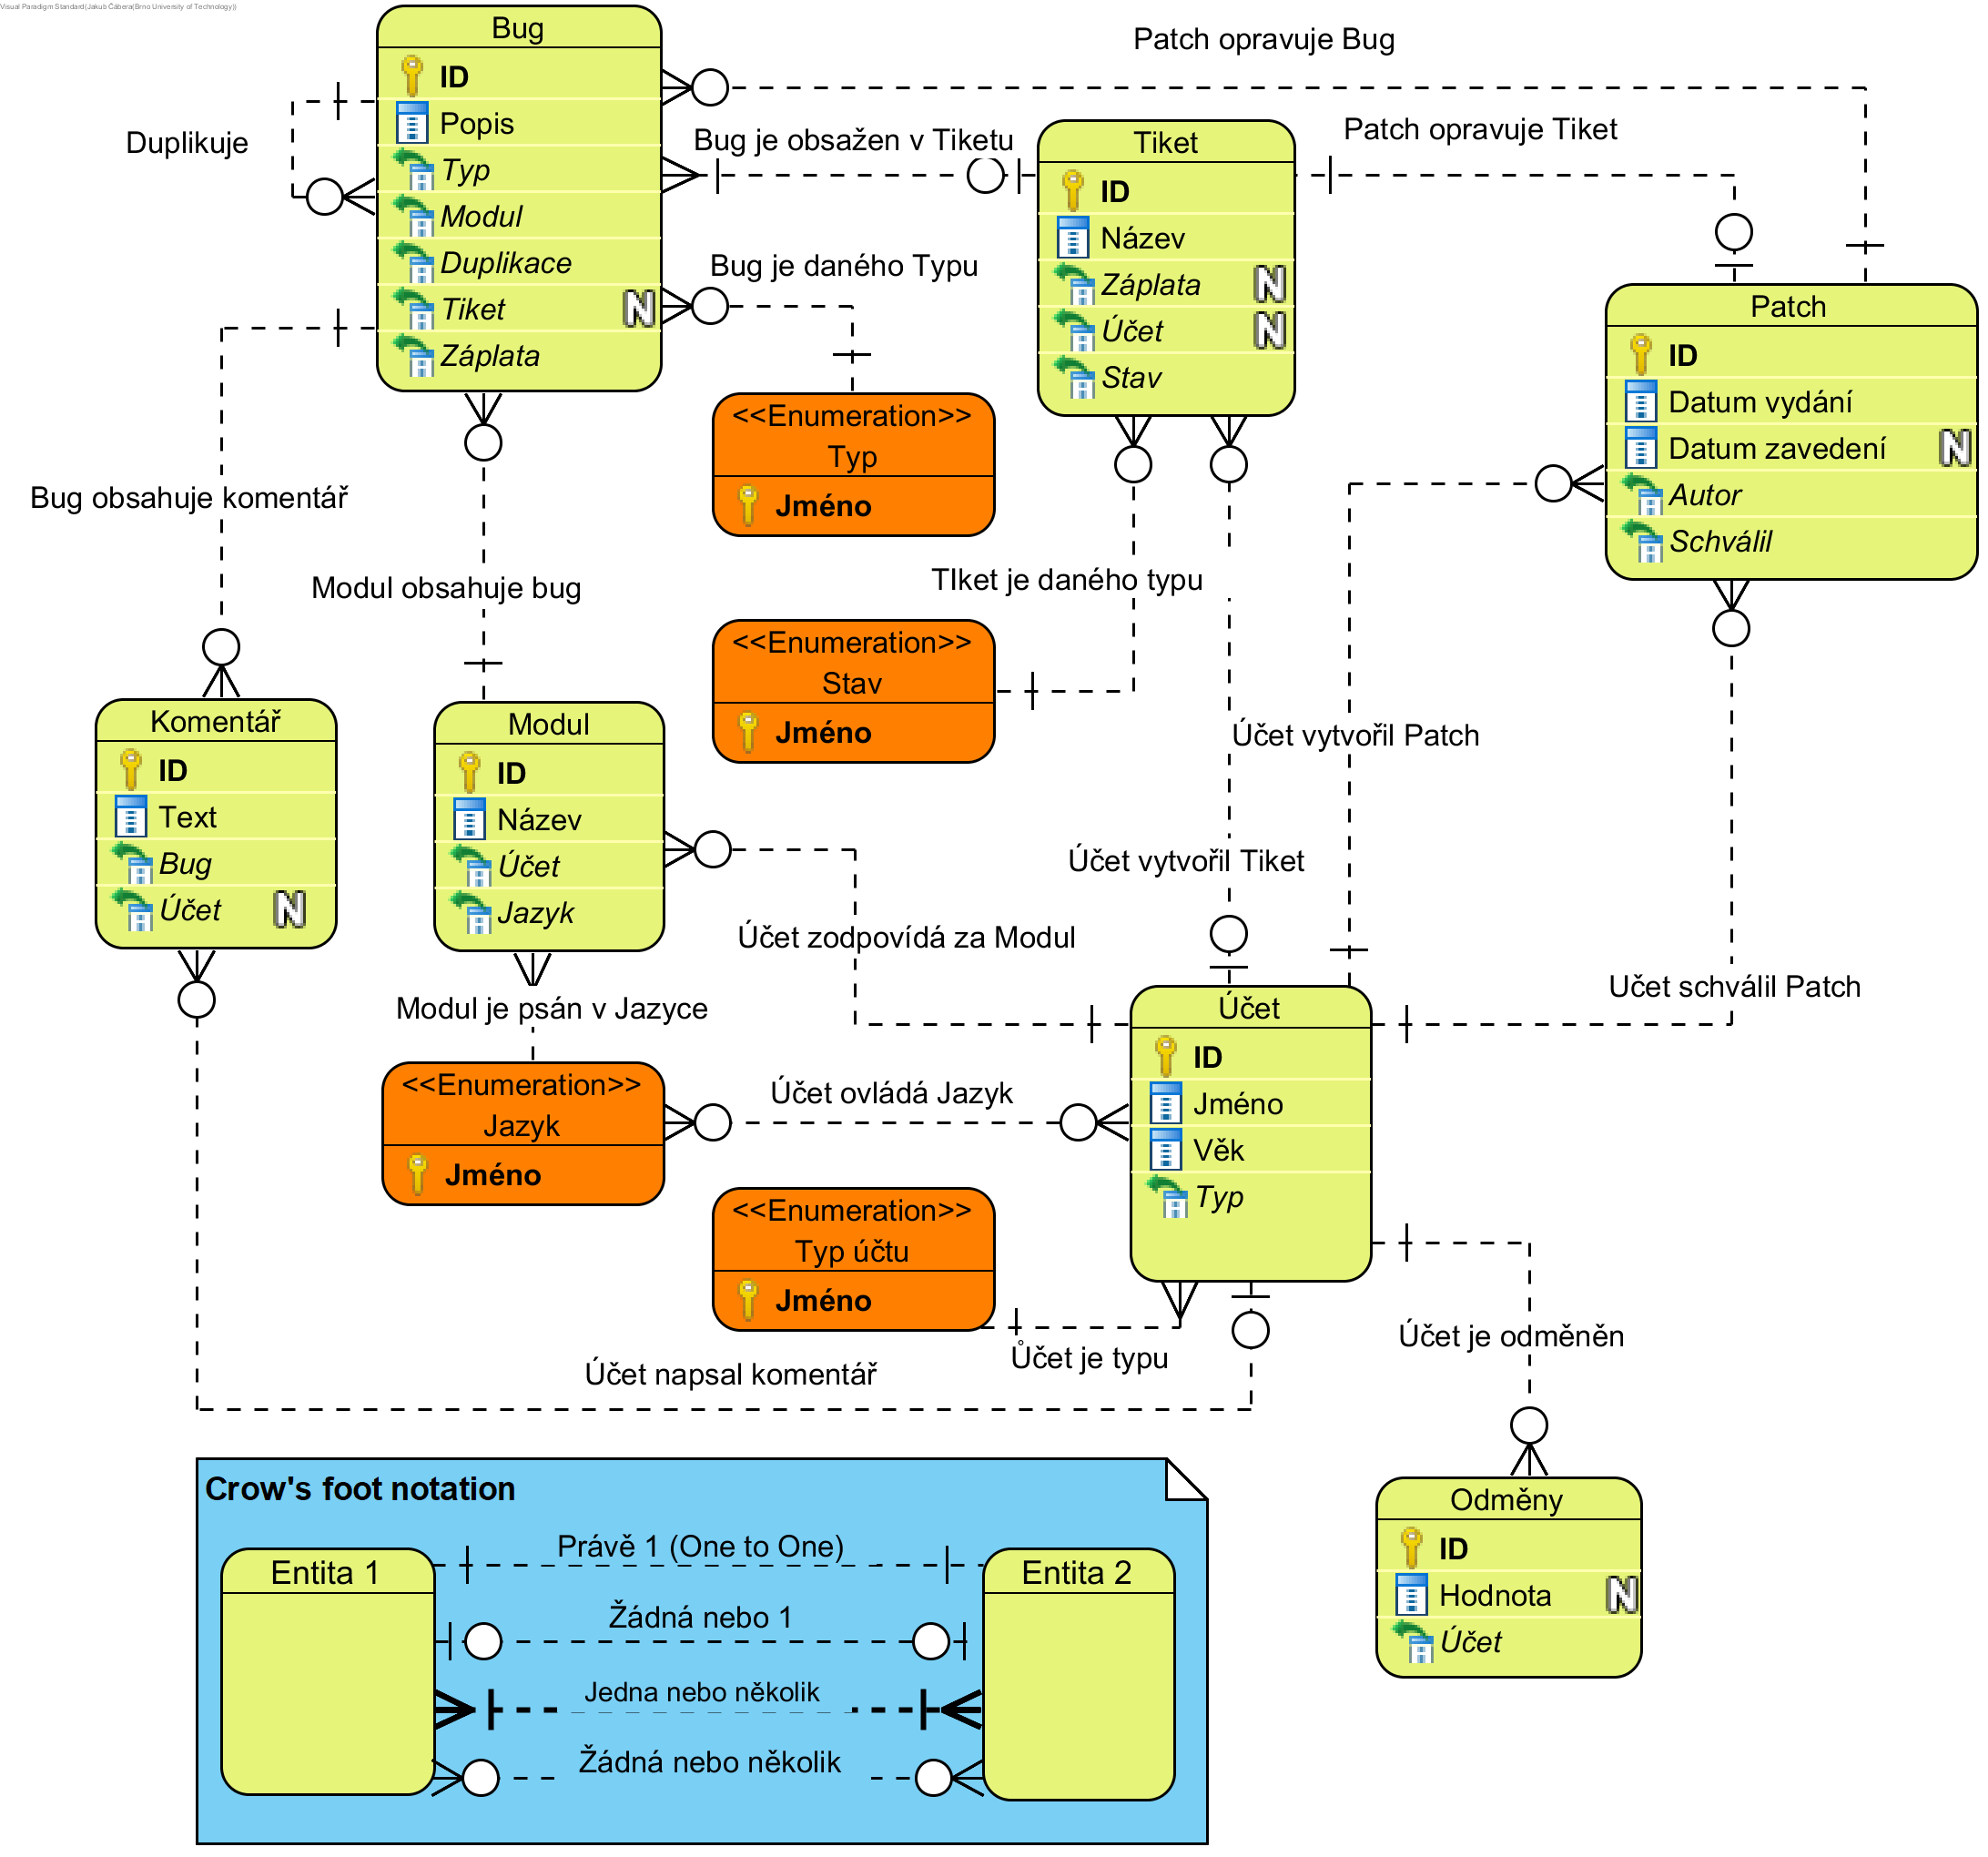
\includegraphics[keepaspectratio]{ER.png}

\end{document}
